\chapter{État de l'Art}
\label{ch:etat_art}

\sommairechapitre

%%%%%%%%%%%%%%%%%%%%%%%%%%%%%%%%%%%%%%%%%%%%%%%%%%%%%%%%%%%%%%%%%
% 2.1. Cadre Théorique de l'Apprenant : Motivation, Intérêt et Pertinence
%%%%%%%%%%%%%%%%%%%%%%%%%%%%%%%%%%%%%%%%%%%%%%%%%%%%%%%%%%%%%%%%%
\section{Cadre Théorique de l'Apprenant : Motivation, Intérêt et Pertinence}
\label{sec:cadre_apprenant}

% ============================================================================
% Sous-section 2.1.1 : Dynamiques Motivationnelles — SDT et CET
% ============================================================================
% Sources : IJCCI_extraction (§2.1), Vault.xlsx
% Calibrage : ~600 mots
% Type : C (Rédaction originale, synthèse analytique)
% ============================================================================

\subsection{Dynamiques Motivationnelles~: SDT et CET}
\label{subsec:SDT_CET}

La motivation intrinsèque --- cette propension à s'engager dans une activité pour le plaisir et la satisfaction qu'elle procure --- constitue un prédicteur robuste de la qualité de l'apprentissage~\citep{deci2000what}. Sa compréhension nécessite d'articuler deux niveaux d'analyse~: les mécanismes par lesquels l'environnement affecte cette motivation, et les besoins psychologiques sous-jacents qui la conditionnent.

Au premier niveau, les facteurs environnementaux n'exercent pas d'effet direct et uniforme sur la motivation~; leur impact dépend de l'interprétation qu'en fait l'individu~\citep{deci1985intrinsic}. Un même feedback peut ainsi être vécu comme \textit{informationnel} --- fournissant un retour constructif sur la compétence et soutenant la motivation --- ou comme \textit{contrôlant} --- exerçant une pression sur le comportement et sapant l'autodétermination. Cette distinction, issue de la Théorie de l'Évaluation Cognitive (CET), s'articule autour de deux dimensions psychologiques~: le \textit{locus de causalité perçu}, soit le sentiment que ses actions émanent de soi plutôt que de contraintes externes, et le \textit{sentiment de compétence}, soit la conviction de pouvoir atteindre les résultats souhaités. Un troisième aspect, \textit{amotivant}, peut signaler l'incompétence et conduire au désengagement total.

Au second niveau, trois besoins psychologiques fondamentaux conditionnent le bien-être et l'engagement~: l'\textit{autonomie}, la \textit{compétence} et l'\textit{affiliation}~\citep{ryan2017self}. La Théorie de l'Autodétermination (SDT) postule que les environnements d'apprentissage favorisent l'intérêt lorsqu'ils satisfont ces besoins à travers des choix significatifs, des défis appropriés, un feedback constructif et des interactions soutenantes. L'ajout du besoin d'affiliation --- le sentiment de connexion aux autres --- étend la portée explicative du modèle au-delà des seules dimensions cognitives pour intégrer la dimension sociale de l'apprentissage.

L'articulation de ces deux niveaux révèle une dynamique complexe~: un environnement qui offre des choix (autonomie), propose des défis calibrés avec un feedback informatif (compétence), et crée des opportunités d'interaction authentique (affiliation), réunit les conditions propices au développement de la motivation intrinsèque. À l'inverse, un environnement perçu comme contrôlant, qui impose des tâches sans en expliciter le sens et isole l'apprenant, tend à éroder cette motivation --- un phénomène particulièrement documenté lors de la transition vers le secondaire~\citep{gnambs2016decline}. Cette période, marquée par une pression accrue sur la performance et des structures scolaires qui peuvent limiter la curiosité naturelle~\citep{engel2011children}, voit la motivation intrinsèque décliner significativement.

Ce déclin revêt une importance particulière pour l'enseignement de l'Histoire, discipline souvent perçue comme distante et déconnectée des expériences personnelles~\citep{audigier2010histoire}. Le défi consiste alors à concevoir des environnements qui, tout en respectant les contraintes curriculaires, créent les conditions de satisfaction des besoins identifiés. Les agents conversationnels offrent une piste prometteuse~: l'interactivité dialogique peut soutenir l'autonomie en permettant à l'élève de diriger l'échange, les réponses adaptatives peuvent nourrir le sentiment de compétence, et les indices sociaux de l'agent peuvent répondre au besoin d'affiliation. Cette hypothèse, qui guide notre programme expérimental, nécessite cependant de comprendre comment l'intérêt se développe et se maintient --- objet de la section suivante.

\subsection{Architecture de l'Intérêt}
\label{subsec:architecture_interet}

L'intérêt, tel que défini dans la recherche en psychologie de l'éducation, combine deux composantes de nature distincte \citep{hidi2006}. La composante affective se manifeste par une expérience positive associée à l'activité --- attention accrue, affect favorable, envie spontanée de poursuivre. La composante cognitive se traduit par une orientation vers la compréhension du contenu : l'individu cherche à approfondir, pose des questions, établit des connexions entre les informations. Cette double nature distingue l'intérêt des construits apparentés. Là où la motivation intrinsèque (cf. \ref{subsec:sdt_cet}) désigne un processus général applicable à toute activité, l'intérêt est toujours dirigé vers un contenu spécifique \citep{renninger2015}. Un même élève peut manifester un intérêt soutenu pour la biologie et un désintérêt marqué pour l'histoire, alors que son niveau de motivation intrinsèque globale reste stable. Cette spécificité de contenu confère à l'intérêt une valeur explicative particulière pour l'apprentissage disciplinaire : il contribue à expliquer pourquoi un dispositif pédagogique efficace dans une matière échoue dans une autre \citep{hidi2000}.

Le développement de l'intérêt suit une séquence en quatre phases dont chacune se caractérise par un équilibre distinct entre soutien externe et engagement autonome \citep{hidi2006}. La première phase, l'intérêt situationnel déclenché, désigne une réponse attentionnelle à un stimulus environnemental --- nouveauté, surprise, incongruité avec les attentes. Cette réponse est brève et dépend entièrement du déclencheur externe. La deuxième phase, l'intérêt situationnel maintenu, apparaît lorsque l'engagement avec le contenu se prolonge au-delà de la réaction initiale : l'apprenant commence à traiter l'information en profondeur, mais le soutien de l'environnement reste nécessaire pour maintenir son attention. La troisième phase, l'intérêt individuel émergent, marque un changement qualitatif : l'apprenant développe une prédisposition à se réengager avec le contenu de sa propre initiative, génère des questions et recherche activement des informations complémentaires. La quatrième phase, l'intérêt individuel développé, correspond à une disposition stable : l'apprenant tolère la frustration, autorégule son apprentissage et produit des questions de curiosité qui alimentent sa progression \citep{renninger2015}. La transition de la deuxième à la troisième phase constitue le point de basculement du modèle : l'intérêt tend à ne plus dépendre du soutien de l'environnement pour devenir auto-entretenu.

Les facteurs qui déclenchent l'intérêt situationnel ne sont pas ceux qui le maintiennent. La nouveauté, le caractère inattendu d'une information et l'intensité perceptive d'un stimulus suffisent à capter l'attention (phase 1), mais leur effet tend à se dissiper si aucune connexion significative ne s'établit avec l'apprenant \citep{hidi2006}. Le maintien de l'intérêt (phase 2) repose sur des facteurs différents : la pertinence personnelle perçue, l'engagement actif dans une tâche signifiante et le sentiment de compétence dans l'interaction avec le contenu \citep{bergin1999}. Le contexte social joue un rôle transversal. L'identité du locuteur, la qualité de la relation avec l'enseignant et l'influence des pairs peuvent à la fois déclencher et maintenir l'intérêt \citep{bergin2016}. Un interlocuteur perçu comme signifiant --- qu'il soit enseignant, pair ou figure de référence --- peut affecter le développement de l'intérêt indépendamment du contenu transmis \citep{renninger2009}. Cette dissociation entre déclenchement et maintien pose un problème de conception : un dispositif qui mise exclusivement sur la nouveauté sans créer de connexion personnelle avec le contenu ne dépasse pas la première phase.

La curiosité et l'intérêt entretiennent une relation de renforcement mutuel qui s'intensifie au fil du développement \citep{hidi2020}. Dans les phases avancées de l'intérêt (phases 3 et 4), l'apprenant ne se contente plus de répondre aux stimuli externes : il génère spontanément des questions qui orientent son exploration du domaine. Ces questions de curiosité constituent le moteur interne de la progression vers un intérêt individuel stable. Les environnements éducatifs qui accueillent ces questions --- plutôt que de les canaliser vers des objectifs prédéterminés --- facilitent la transition entre les phases \citep{renninger2015}. La progression de l'intérêt situationnel vers l'intérêt individuel dépend toutefois d'un facteur que le modèle identifie sans l'approfondir : la capacité de l'apprenant à percevoir le contenu comme personnellement pertinent. Ce mécanisme, par lequel un savoir disciplinaire acquiert une valeur aux yeux de l'apprenant, relève d'un cadre théorique distinct : la théorie de la valeur et de la pertinence, qui fait l'objet de la section suivante.

\subsection{Pertinence, Valeur et Personnalisation}
\label{subsec:pertinence_valeur}

La section précédente a identifié la pertinence personnelle comme levier de la progression de l'intérêt situationnel vers l'intérêt individuel. La théorie de l'attente-valeur (\textit{Expectancy-Value Theory}, EVT) fournit le cadre qui explique ce mécanisme. L'engagement d'un apprenant dans une tâche dépend de deux évaluations simultanées : l'attente de succès (la croyance de pouvoir réussir) et la valeur subjective attribuée à la tâche \citep{wigfield1998}. La valeur se décompose en quatre dimensions : la valeur intrinsèque (le plaisir retiré de l'activité, qui correspond à l'intérêt tel que défini en \ref{subsec:architecture_interet}), la valeur d'utilité (l'utilité perçue du contenu pour des buts futurs), la valeur d'atteinte (l'importance de la réussite pour l'image de soi) et le coût (l'effort requis, l'anxiété générée, les activités alternatives sacrifiées). La pertinence personnelle constitue le mécanisme transversal par lequel ces dimensions s'activent : elle désigne le degré auquel l'apprenant perçoit une connexion entre le contenu et sa propre vie, ses buts ou son identité \citep{albrecht2018}. Ce construit ne se réduit pas à l'utilité perçue. Il forme un continuum qui va de l'association ponctuelle (un exemple qui rappelle une expérience vécue) à l'identification profonde (un contenu qui touche aux valeurs ou aux aspirations de l'individu) \citep{priniski2018}.

Les interventions qui visent à renforcer la valeur d'utilité perçue illustrent comment la pertinence peut être activée en contexte scolaire. L'approche consiste à demander aux élèves de rédiger un texte reliant le contenu du cours à leur vie quotidienne --- non pas à leur transmettre des arguments sur l'utilité de la matière, mais à les amener à construire eux-mêmes cette connexion. En sciences, cette intervention tend à augmenter l'intérêt et la performance, avec un effet plus marqué chez les élèves dont les attentes de succès sont initialement faibles \citep{hulleman2009}. Le mécanisme est actif : l'apprenant ne reçoit pas passivement une information sur la valeur du contenu, il la construit par un effort de mise en relation. Quatre leviers d'intervention ont été identifiés pour soutenir ce processus : adapter les caractéristiques structurelles de l'environnement d'apprentissage, personnaliser le contexte, proposer un apprentissage par problèmes et souligner l'utilité du contenu \citep{harackiewicz2016}. Ces leviers opèrent sur le passage de l'intérêt situationnel déclenché à l'intérêt situationnel maintenu (cf. \ref{subsec:architecture_interet}) : ils transforment une réaction attentionnelle initiale en engagement prolongé en ancrant le contenu dans l'expérience de l'apprenant.

La personnalisation de l'apprentissage constitue la traduction pédagogique du principe de pertinence. Trois mécanismes distincts semblent contribuer indépendamment à la motivation : la contextualisation (ancrer le contenu dans des situations familières à l'apprenant), la personnalisation proprement dite (intégrer des éléments liés à l'identité de l'élève --- son prénom, ses centres d'intérêt) et le choix (offrir des options qui permettent à l'apprenant de connecter le contenu à ses préférences) \citep{cordova1996}. Le contrôle sur des éléments même non essentiels à la tâche --- choix d'un avatar, d'un thème visuel --- tend à augmenter la motivation, ce qui rejoint le besoin d'autonomie identifié par la SDT (cf. \ref{subsec:sdt_cet}). Les interventions ciblant les intérêts individuels tendent à augmenter l'engagement dans des matières perçues comme difficiles \citep{reber2018}. Le choix d'exemples pertinents renforce l'engagement, en particulier chez les élèves dont l'intérêt initial est faible \citep{hogheim2015}. L'intégration des questions formulées par les élèves dans le curriculum produit des effets comparables, en plaçant la curiosité de l'apprenant au centre du dispositif pédagogique \citep{hagay2015}.

La personnalisation se heurte toutefois à des contraintes qui limitent sa mise en œuvre à grande échelle. Trois obstacles ont été identifiés : la diversité des intérêts au sein d'une même classe, l'évolution de ces intérêts dans le temps et le coût de production de contenus personnalisés de qualité pour chaque élève \citep{walkington2018}. Ces contraintes rendent la personnalisation manuelle difficilement généralisable, ce qui justifie la recherche de dispositifs capables d'adapter le contenu de manière automatisée. La pertinence et la personnalisation expliquent \textit{pourquoi} un apprenant s'engage avec un contenu donné. La question complémentaire --- \textit{comment} la modalité d'interaction avec ce contenu détermine la profondeur de l'apprentissage --- relève d'un cadre distinct : le modèle ICAP, qui fait l'objet de la section suivante.

% ============================================================================
% Sous-section 2.1.4 : L'Apprentissage Actif et le Cadre ICAP
% ============================================================================
% Sources : IJCCI_extraction (§2.3), Chi (2009), Freeman et al. (2014)
% Calibrage : ~550 mots
% Type : C (Rédaction originale)
% ============================================================================

\subsection{L'Apprentissage Actif et le Cadre ICAP}
\label{subsec:ICAP}

Les sections précédentes ont montré que l'effort cognitif investi dans la génération de connexions personnelles renforce leur impact motivationnel. Ce constat s'inscrit dans un cadre plus général~: l'apprentissage actif, qui dépasse la simple activité physique pour désigner le fait de \og penser activement à ce que l'on fait\fg{}~\citep{mayer2014cambridge, yannier2021active}. La question devient alors~: comment caractériser les différents niveaux d'engagement cognitif et prédire leurs effets sur l'apprentissage?

Le cadre ICAP (\textit{Interactive, Constructive, Active, Passive}) propose une taxonomie hiérarchisée des activités d'apprentissage selon leur niveau d'engagement cognitif~\citep{chi2009active}. Le mode \textit{Passif} correspond à la réception d'information sans comportement observable au-delà de l'attention --- écouter un cours, regarder une vidéo. Le mode \textit{Actif} implique une manipulation ou une attention focalisée sans production de nouvelles idées --- prendre des notes verbatim, surligner. Le mode \textit{Constructif} requiert la génération d'idées qui dépassent l'information présentée --- formuler des hypothèses, élaborer des explications, connecter le contenu à son expérience personnelle. Le mode \textit{Interactif} ajoute une dimension dialogique~: les partenaires co-construisent des connaissances à travers un échange où chacun contribue substantiellement.

La prédiction centrale du modèle --- Interactif $>$ Constructif $>$ Actif $>$ Passif en termes de gains d'apprentissage --- a reçu un soutien empirique substantiel. Une méta-analyse portant sur 225 études montre que l'apprentissage actif augmente significativement la performance des étudiants en STIM comparé aux cours magistraux~\citep{freeman2014active}. L'interactivité permet de réguler le rythme d'apprentissage, d'explorer les concepts selon ses intérêts, de formuler des questions et de recevoir un feedback immédiat~\citep{domagk2010pedagogical, evans2007interactivity}.

Cette hiérarchie éclaire les résultats sur les interventions de pertinence~: les approches à effort élevé (auto-génération, réévaluation dirigée) relèvent du mode \textit{Constructif}, tandis que les approches à faible effort (communication directe) maintiennent l'apprenant en mode \textit{Passif}. L'efficacité supérieure des premières s'explique ainsi par leur niveau d'engagement cognitif plus profond. Un paradoxe mérite cependant attention~: l'apprentissage actif, bien que conduisant à de meilleurs résultats, est souvent perçu comme moins efficace par les apprenants eux-mêmes~\citep{deslauriers2019measuring}. L'effort cognitif accru est interprété comme un signe de difficulté alors qu'il indique un traitement plus profond.

Dans l'enseignement de l'Histoire, les approches interactives produisent des effets positifs sur la compréhension et l'intérêt. Les discussions de groupe favorisent une meilleure compréhension des concepts historiques~\citep{delfavero2007classroom}. La narration numérique interactive, avec des points de décision stratégiques, stimule des discussions significatives et une compréhension plus profonde~\citep{petousi2022interactive}. La combinaison d'interactions tangibles avec des récits émotionnels encourage les adolescents à s'engager avec les figures historiques au-delà de la connaissance factuelle~\citep{roussou2024emotions}.

Un agent conversationnel incarnant un personnage historique se situe naturellement au niveau \textit{Interactif}~: l'élève formule des questions (activité constructive), l'agent répond, et l'échange peut conduire à une co-construction de sens. Cette position contraste avec la vidéo (mode \textit{Passif}) et le texte (mode \textit{Actif} si l'élève surligne ou prend des notes). Le cadre ICAP prédit ainsi que l'agent dialogique devrait produire des gains d'engagement et d'apprentissage supérieurs aux formats traditionnels --- une prédiction que notre programme expérimental vise à tester.

Cette convergence des cadres théoriques --- SDT, développement de l'intérêt, théorie de l'attente-valeur, ICAP --- dessine les contours d'une intervention prometteuse~: un agent conversationnel qui satisfait les besoins d'autonomie, de compétence et d'affiliation, déclenche et maintient l'intérêt par la nouveauté et l'interaction sociale, permet la génération de connexions personnelles, et engage l'apprenant au niveau interactif du cadre ICAP.


%%%%%%%%%%%%%%%%%%%%%%%%%%%%%%%%%%%%%%%%%%%%%%%%%%%%%%%%%%%%%%%%%
% 2.2. Le Contexte Disciplinaire : Enseigner et Apprendre l'Histoire
%%%%%%%%%%%%%%%%%%%%%%%%%%%%%%%%%%%%%%%%%%%%%%%%%%%%%%%%%%%%%%%%%
\section{Le Contexte Disciplinaire : Enseigner et Apprendre l'Histoire}
\label{sec:contexte_histoire}

\subsection{Le Triple Décalage de l'Histoire Scolaire}
\label{subsec:triple_decalage}

L'histoire en tant que discipline académique repose sur un processus d'enquête interprétative : le chercheur confronte des sources de natures diverses, reconstruit des contextes disparus et produit des récits qui rendent compte de la complexité du passé \citep{wineburg1991}. L'enseignement scolaire de cette discipline opère cependant une réduction systématique de cette complexité. Les manuels présentent un récit unique, linéaire, sans auteur apparent --- comme si les événements se racontaient d'eux-mêmes. Les sources primaires, lorsqu'elles apparaissent, servent d'illustrations plutôt que de matériaux d'enquête. Les élèves ne sont pas formés à lire un document comme un \textit{site d'interprétation} où se croisent intentions, contextes de production et silences \citep{wineburg1991}. Ce premier décalage, entre la nature épistémologique de la discipline et sa transposition scolaire, affecte directement la perception que les élèves construisent de la matière : l'histoire apparaît comme un répertoire de faits à mémoriser plutôt que comme un processus de construction de sens.

Le deuxième décalage concerne la valeur perçue de la discipline. Les élèves reconnaissent généralement l'importance sociale de l'histoire --- formation du citoyen, compréhension du présent, construction de l'identité collective --- mais perçoivent son enseignement comme déconnecté de leur expérience personnelle \citep{audigier2010}. Ce paradoxe s'analyse par le prisme de la théorie de l'attente-valeur (cf.~\ref{subsec:pertinence_valeur}) : la valeur d'atteinte (l'importance de l'histoire pour l'identité sociale) coexiste avec un déficit de valeur d'utilité (aucune application professionnelle immédiate perçue) et de valeur intrinsèque (peu de plaisir retiré de l'activité scolaire). Les disciplines scientifiques et technologiques bénéficient d'une utilité professionnelle visible qui facilite la construction de la pertinence ; l'histoire exige un travail de connexion personnelle que ni le programme ni le format pédagogique dominant ne facilitent. Ce décalage perceptif s'accentue au secondaire, au moment où le besoin d'autonomie de l'adolescent entre en conflit avec un enseignement prescriptif qui laisse peu de place aux questions de l'élève (cf.~\ref{subsec:sdt_cet}).

Le troisième décalage oppose le potentiel narratif de la discipline à la pauvreté des formats pédagogiques qui la transmettent. L'histoire possède une richesse intrinsèque --- personnages, conflits, dilemmes moraux, tournants imprévisibles --- qui la prédispose à l'engagement émotionnel et à la construction de sens. Pourtant, le format transmissif dominant (cours magistral, lecture de manuels, prise de notes) neutralise ce potentiel en plaçant l'élève en mode passif au sens du cadre ICAP (cf.~\ref{subsec:icap}). L'enseignement reste dominé par la monomodalité textuelle : les enseignants eux-mêmes peinent à concevoir les sources historiques autrement que comme des textes écrits \citep{wineburg1991}. La personnalisation, identifiée comme levier de pertinence (cf.~\ref{subsec:pertinence_valeur}), se heurte aux contraintes logistiques de classes nombreuses et de programmes denses. Des pratiques pédagogiques émergentes cherchent à résoudre simultanément ces trois décalages en combinant engagement actif, connexion personnelle et accès multimodal au passé --- elles font l'objet des sections suivantes.

\subsection{Les Pratiques Actives en Histoire : Au-Delà du Cours Magistral}
\label{subsec:pratiques_actives}

Les recherches en didactique de l'histoire ont identifié des formats pédagogiques qui déplacent l'élève de la réception passive d'un récit vers la construction active de sa compréhension. La discussion collaborative et la résolution de problèmes en groupe augmentent la compréhension des concepts historiques et l'intérêt pour la discipline par rapport à l'apprentissage individuel : les échanges entre pairs obligent chaque participant à expliciter son raisonnement, à confronter ses interprétations et à intégrer des perspectives divergentes \citep{delfavero2007}. Le récit interactif numérique, dans lequel les apprenants rencontrent des points de décision stratégiques au fil d'une narration historique, produit un effet convergent : les choix narratifs stimulent la discussion de groupe et favorisent une compréhension en profondeur des enjeux historiques, parce qu'ils contraignent l'apprenant à évaluer les conséquences de décisions prises dans un contexte passé \citep{petousi2022}.

L'immersion dans des environnements virtuels renforce ces effets en ajoutant une dimension spatiale et sensorielle à l'expérience historique. La reconstruction tridimensionnelle de cités antiques améliore la performance et l'engagement des élèves, qui consacrent davantage de temps à l'exploration du contenu historique que les groupes exposés au même contenu par le texte ou la vidéo \citep{ijaz2017}. Les dispositifs muséaux interactifs, qui combinent objets tangibles et récits à forte charge émotionnelle, favorisent l'empathie historique et la pensée critique chez les adolescents : la manipulation physique d'artefacts liés à des récits personnels du passé crée une connexion affective que le texte seul ne parvient pas à produire \citep{roussou2024}. Ces résultats convergent vers un principe commun : l'apprentissage de l'histoire gagne en profondeur lorsque l'élève passe de la réception d'un récit clos à la construction active de sa propre compréhension du passé --- un déplacement qui correspond au passage du mode passif vers les modes constructif et interactif du cadre ICAP (cf.~\ref{subsec:icap}). Trois formats illustrent ce principe avec une force particulière : la simulation, l'incarnation par le jeu de rôle et la multimodalité du jeu historique.

% ============================================================================
% Sous-section 2.2.3 : Leviers Pédagogiques de l'Engagement
% ============================================================================
% Sources : État de l'Art Histoire (Harris & Haydn 2006, Gómez Carrasco et al. 2021,
%           Cairns & Garrard 2024, Van Straaten et al. 2015, Bergin 1999,
%           Henkaline 2023)
% Calibrage : ~650 mots
% Type : C (Rédaction originale)
% ============================================================================

\subsection{Leviers Pédagogiques de l'Engagement}
\label{subsec:pratiques_pedagogiques}

Si le paradoxe \og pertinent mais ennuyeux\fg{} désigne le problème, la recherche en didactique de l'histoire identifie avec une précision croissante les conditions de sa résolution. Les données empiriques convergent vers un constat structurant~: l'efficacité pédagogique dépend moins du contenu enseigné que des modalités d'enseignement.

Les méthodes interactives recueillent massivement l'adhésion des élèves. Sur 1740 répondants britanniques, le jeu de rôle et le théâtre totalisent 295 mentions positives, les discussions et débats 108, le travail de groupe 56~\citep{harris2006pupils}. À l'inverse, le travail écrit excessif concentre 394 mentions négatives, les tests fréquents 151, la sur-utilisation des manuels et fiches 57. Ce pattern n'est pas propre au contexte britannique~: les élèves américains valorisent de même les méthodes expérientielles~--- simulations de procès, vidéos immersives~--- et critiquent la prise de notes passive~\citep{henkaline2023eighth}. La convergence transculturelle de ces préférences suggère qu'elles reflètent des invariants cognitifs plutôt que des spécificités locales.

Ces préférences ne relèvent pas du simple confort~; elles produisent des gains mesurables sur l'apprentissage. Un programme de formation combinant méthodes actives et réflexion épistémologique, évalué auprès de 467 élèves répartis en 18 classes, révèle des améliorations significatives~: $r = 0.522$ pour l'évaluation de la méthodologie, $r = 0.443$ pour la motivation, $r = 0.335$ pour l'apprentissage perçu~\citep{gomezcarrasco2021motivation}. L'intensité de l'intervention module les effets~: les enseignants formés de manière approfondie produisent des résultats supérieurs à ceux formés superficiellement. La transformation pédagogique requiert donc un investissement substantiel en formation.

Le cadre ICAP (cf.~\S\ref{subsec:ICAP}) éclaire les mécanismes sous-jacents à cette efficacité. Les méthodes interactives~--- débats, jeux de rôle, confrontation des interprétations~--- activent les modes \textit{Constructif} et \textit{Interactif}, où l'élève génère des inférences et co-construit du sens avec ses pairs. Le cours magistral cantonne l'élève au mode \textit{Passif}, où l'attention ne garantit pas le traitement profond. La supériorité des méthodes actives n'est donc pas une question de préférence subjective mais de fonctionnement cognitif~: l'engagement émotionnel améliore la mémorisation, l'expérience directe développe l'empathie historique, l'interaction sociale répond aux besoins d'appartenance~\citep{bergin1999influences}.

Parmi les leviers identifiés, la connexion explicite entre temporalités occupe une place centrale. Un cadre théorique articulant passé, présent et futur comme condition de la pertinence perçue montre que les élèves trouvent les tâches de connexion temporelle plus difficiles mais plus intéressantes que les exercices traditionnels~\citep{vanstraaten2015making}. Cette observation trouve un écho dans les données australiennes~: les élèves qui poursuivent l'histoire valorisent précisément sa capacité à éclairer le présent~\citep{cairns2024learning}. L'explicitation de ces connexions~--- plutôt que leur découverte supposée spontanée~--- constitue une condition de l'engagement.

L'enseignant demeure la variable déterminante. Les écarts d'appréciation entre établissements (cf.~\S\ref{subsec:perception_eleves}) ne s'expliquent ni par les contenus enseignés ni par les caractéristiques des publics, mais par les pratiques professorales et départementales. Les enseignants \og enthousiastes qui respectent les élèves\fg{} obtiennent de meilleurs résultats indépendamment des méthodes utilisées~\citep{harris2006pupils}. Cette observation s'inscrit dans un modèle plus général de l'intérêt situationnel~: nouveauté modérée, interaction sociale, narration, prise en compte de l'appartenance culturelle constituent autant de facteurs que l'enseignant contrôle et qui peuvent déclencher l'intérêt même chez des élèves initialement peu motivés~\citep{bergin1999influences}.

Ces résultats dessinent le cahier des charges implicite d'une innovation pédagogique en histoire. L'efficacité suppose l'activation de l'élève plutôt que sa réception passive, la confrontation des perspectives plutôt que la transmission d'un récit unique, la connexion explicite aux préoccupations contemporaines plutôt que l'enfermement dans le passé. Les sections suivantes examinent dans quelle mesure les technologies d'interaction~--- et singulièrement les agents conversationnels~--- peuvent satisfaire ces exigences.


%%%%%%%%%%%%%%%%%%%%%%%%%%%%%%%%%%%%%%%%%%%%%%%%%%%%%%%%%%%%%%%%%
% 2.3. Cadre Théorique de l'Interaction : Cognition, Multimédia et Présence Sociale
%%%%%%%%%%%%%%%%%%%%%%%%%%%%%%%%%%%%%%%%%%%%%%%%%%%%%%%%%%%%%%%%%
\section{Cadre Théorique de l'Interaction : Cognition, Multimédia et Présence Sociale}
\label{sec:cadre_interaction}

\subsection{Architecture cognitive et apprentissage multimédia}
\label{subsec:architecture_cognitive}

Tout agent pédagogique opère dans les limites de la mémoire de travail. La théorie de la charge cognitive identifie cette contrainte : la mémoire de travail ne traite qu'un nombre restreint d'éléments simultanément \citep{sweller1988}. Trois types de charge se partagent cette capacité. La charge intrinsèque dépend de la complexité du contenu et du niveau de l'apprenant. La charge extrinsèque résulte d'un design inadapté : informations redondantes, navigation confuse, éléments visuels non pertinents. La charge pertinente (\textit{germane load}) correspond à l'effort consacré à la construction de schémas mentaux \citep{sweller2011}. Ces trois charges ne sont pas indépendantes : réduire la charge extrinsèque libère des ressources pour la charge pertinente. L'enjeu du design d'un agent pédagogique se formule dans ces termes : minimiser la charge extrinsèque pour maximiser les ressources disponibles à l'apprentissage.

La théorie cognitive de l'apprentissage multimédia (CTML) prolonge ce cadre en précisant comment l'information est traitée quand elle combine texte, image et son \citep{mayer2020}. Trois hypothèses structurent le modèle. L'information entre par deux canaux distincts (visuel et auditif). Chaque canal a une capacité limitée. L'apprentissage requiert un traitement actif : sélection, organisation et intégration de l'information avec les connaissances antérieures. De ces hypothèses découlent des principes de design applicables aux agents pédagogiques. Le principe de modalité établit qu'une narration orale accompagnant une image produit un meilleur apprentissage qu'un texte écrit accompagnant la même image. La narration répartit la charge entre les deux canaux au lieu de surcharger le seul canal visuel. Le principe de redondance montre, à l'inverse, que présenter simultanément un texte écrit et une narration identique tend à dégrader la performance. Le canal visuel traite alors à la fois le texte et l'image, ce qui génère une charge extrinsèque. Ces principes reposent cependant sur des conditions expérimentales précises. Ils supposent un contenu technique accompagné de schémas, un apprenant novice et une présentation linéaire. Leur transposition aux interactions conversationnelles, où l'apprenant contrôle le rythme et le contenu des échanges, n'est pas directement validée. Le principe de modalité fournit néanmoins la justification technique des agents oraux : un agent qui parle libère le canal visuel pour les contenus graphiques que l'apprenant doit analyser --- cartes, schémas, documents historiques \citep{mayer2014-ju}.

Ces principes traitent l'apprenant comme un système de traitement de l'information. L'optimisation des canaux cognitifs explique \textit{comment} l'information est encodée, mais pas \textit{pourquoi} un apprenant consentirait à fournir l'effort nécessaire. La CTML, dans sa formulation initiale, ne distingue pas un agent pédagogique d'un diaporama narré. Les deux exploitent le canal auditif de la même manière. L'extension du modèle vers les indices sociaux (\textit{social cues hypothesis}) comble cette lacune \citep{mayer2014-ju}. Certains signaux --- voix humaine, visage expressif, regard dirigé --- déclenchent un sentiment de présence sociale. Ce sentiment transforme le traitement d'information en échange interpersonnel. L'artefact numérique active alors des réponses ordinairement réservées aux interactions humaines. Le mécanisme psychologique qui sous-tend cette activation fait l'objet de la section suivante.


\subsection{La présence sociale et le paradigme CASA}
\label{subsec:presence_sociale_CASA}

La présence sociale désigne le sentiment subjectif d'être en présence d'une autre entité intelligente \citep{biocca2003}. Ce construit comporte trois dimensions. La co-présence désigne la perception qu'un autre être partage le même espace. L'implication psychologique renvoie à l'attention portée à cet être. L'engagement comportemental correspond à la tendance à interagir avec lui. La présence sociale n'est pas une propriété de la technologie. Un même agent peut susciter un fort sentiment de présence chez un apprenant et aucun chez un autre, selon le contexte, les attentes et la qualité des indices sociaux. Ce point est décisif pour le design pédagogique : la question n'est pas de savoir si un agent \textit{est} social, mais s'il \textit{est perçu} comme tel.

Le paradigme CASA (\textit{Computers Are Social Actors}) explique comment cette perception émerge. Les travaux fondateurs montrent que les utilisateurs appliquent spontanément aux ordinateurs des règles réservées aux interactions humaines : politesse, réciprocité, attribution de traits de personnalité \citep{nass1994}. Un ordinateur qui se présente comme un ``partenaire d'équipe'' reçoit des évaluations plus favorables qu'un ordinateur neutre --- alors même que les participants déclarent savoir qu'il s'agit d'une machine \citep{nass2000}. Le mécanisme en jeu n'est pas une croyance consciente dans l'humanité de la machine. Il relève de ce que Nass nomme \textit{mindlessness} : l'activation automatique de scripts sociaux en réponse à des indices minimaux. La présence d'une voix, d'un nom ou d'un tour de parole suffit à déclencher ces réponses.

Les conséquences pour l'apprentissage découlent directement de ce mécanisme. Si l'apprenant traite l'agent comme un partenaire social, il s'engage dans un contrat conversationnel implicite : effort accru pour comprendre le message, traitement plus profond de l'information, volonté de réciprocité dans l'échange. La théorie de l'agence sociale formalise cette chaîne causale : les indices sociaux activent la présence sociale, qui génère un partenariat perçu, lequel augmente l'effort cognitif et améliore l'apprentissage \citep{mayer2012}. La perception d'un interlocuteur transforme un exercice de traitement d'information en échange social --- un déplacement qui peut faciliter la transition vers le mode interactif du cadre ICAP (cf.~\ref{subsec:icap}), où l'apprenant co-construit le savoir plutôt que de le recevoir.

L'intensité de la présence sociale varie avec le degré d'anthropomorphisme de l'agent. La tendance humaine à attribuer des caractéristiques humaines aux entités non humaines suit un gradient : plus un agent présente d'indices humains, plus il est perçu comme doté d'intentions et de compétences \citep{epley2007}. Ce gradient s'observe empiriquement dans un continuum qui va du texte seul à un agent doté d'une voix, d'un visage et d'un corps \citep{gong2008}. L'attribution ne se limite pas à la compétence : les apprenants projettent sur l'agent des intentions, des émotions et une personnalité, ce qui produit un investissement émotionnel dans le processus d'apprentissage \citep{kim2006}. Chaque ajout d'indice social augmente la crédibilité perçue et la confiance accordée à l'agent \citep{li2023}. La congruence entre l'apparence de l'agent et le contenu enseigné constitue un facteur supplémentaire : un agent thématiquement aligné avec le domaine --- par exemple un astronaute enseignant l'astronomie --- génère une présence sociale et un engagement supérieurs à ceux d'un agent générique \citep{schmidt2019-et}. Cette hypothèse de congruence se heurte cependant à des résultats contradictoires. Une étude manipulant la tenue vestimentaire d'un agent (appropriée vs formelle) et le décor de la vidéo (atelier vs salon) n'observe aucun effet principal de ces facteurs sur l'apprentissage \citep{decker2023-ss}. Une interaction inattendue émerge : la combinaison tenue appropriée et décor inapproprié produit les meilleurs résultats, avec une taille d'effet faible ($\eta^2_p = 0{,}02$). La tenue appropriée augmente la crédibilité perçue sans affecter l'expertise perçue. Ces données suggèrent que l'effet de congruence thématique ne se généralise pas systématiquement aux aspects vestimentaires et contextuels : le type d'alignement --- thématique, vestimentaire ou environnemental --- pourrait moduler différemment la perception de l'agent et son efficacité pédagogique.


\subsection{De la présence à l'apprentissage : incarnation et agence sociale}
\label{subsec:incarnation_agence_sociale}

La chaîne causale proposée par la théorie de l'agence sociale comporte quatre maillons : les indices sociaux (voix, visage, gestes) activent la présence sociale, qui génère la perception d'un partenariat, laquelle augmente l'effort de traitement et améliore l'apprentissage en profondeur \citep{moreno2001-th, mayer2012}. Ce modèle se distingue de la CTML (cf.~\ref{subsec:architecture_cognitive}) sur un point précis. Le gain d'apprentissage ne résulte pas d'une répartition optimale de l'information entre canaux cognitifs. Il résulte d'une motivation sociale à traiter le contenu plus en profondeur. Deux décennies de recherche confirment cette prédiction, tout en révélant que la nature des indices sociaux détermine l'ampleur du bénéfice \citep{veletsianos2014, johnsonlester2016}. Parmi ces indices, la voix constitue le signal le plus robuste.

La perception d'une voix humaine peut suffire à déclencher l'attribution d'un esprit à l'agent : l'auditeur infère des intentions, des émotions et une capacité de compréhension \citep{schroeder2016}. En contexte d'apprentissage, la voix humaine surpasse la voix synthétique sur les mesures de transfert et de compréhension, sans effet systématique sur la rétention factuelle \citep{craig2017}. Plusieurs méta-analyses confirment cette hiérarchie à travers des contextes variés \citep{davis2018, wang2023-meta}. La combinaison d'émotions positives et de caractéristiques vocales humaines renforce la motivation \citep{wang2021}. La prosodie --- variations de hauteur, de rythme et d'intensité --- contribue indépendamment de la qualité vocale \citep{ehret2021}. Les indices prosodiques pèsent davantage que les indices visuels dans la construction du sentiment de présence sociale. Une voix synthétique monotone peut annuler le bénéfice d'un visage expressif \citep{craig2019, chiou2020}. Des données récentes d'oculométrie confirment cette hiérarchie : la combinaison voix humaine et apparence formelle oriente l'attention vers le contenu plutôt que vers l'agent, tout en réduisant la charge cognitive \citep{xiao2025}. La qualité vocale produit un rendement supérieur à celui du raffinement visuel.

Si la voix constitue le signal le plus robuste, la composante visuelle produit des résultats plus incertains. La présence d'un corps ou d'un visage à l'écran contribue au sentiment de présence sociale et renforce l'implication émotionnelle \citep{sanghoon2015, alemdag2022-rc}. L'apparence de l'agent influence la perception de compétence et l'attitude envers le contenu \citep{domagk2010}. Un agent visible améliore le transfert par rapport à une narration seule \citep{mayer2012}. Cet avantage n'est cependant pas consistant. La majorité des études ne trouvent pas de différence d'apprentissage attribuable à la seule présence visuelle \citep{heidig2011, wangruiz2021}. Les agents en 2D produisent des résultats supérieurs à ceux en 3D \citep{castro-Alonso2021-qh}. Le réalisme géométrique ne détermine pas l'efficacité pédagogique. L'apparence agit sur les variables perceptuelles --- présence sociale, engagement, satisfaction --- sans améliorer de manière consistante l'apprentissage mesuré. L'affect lié à l'apparence constitue un facteur distinct : les agents dotés d'expressions émotionnelles améliorent la motivation et la rétention, ce qui suggère que l'effet ne transite pas par le réalisme mais par la résonance affective \citep{guo2015, shiban2015-fe}.

La distinction entre propriétés externes et internes des agents éclaire ce paradoxe \citep{moreno2004}. Les propriétés externes --- image et voix --- constituent la persona de l'agent. Les propriétés internes désignent les méthodes pédagogiques : feedback, guidage, modélisation. Les travaux conduits avec Herman The Bug, un personnage 2D enseignant la botanique, ont permis d'isoler ces dimensions \citep{lester1999}. La présence visuelle de l'agent n'affecte pas l'apprentissage lorsque les méthodes pédagogiques restent constantes. La voix suffit à activer la perception d'un partenaire. L'image, en l'absence de valeur pédagogique ajoutée, reste un \textit{seductive detail} --- un élément engageant mais non fonctionnel pour l'apprentissage \citep{harp1998, rey2012}. Les caractéristiques de persona --- apparence, genre, voix, expressions, mouvements --- interagissent de manière complexe et produisent des effets différenciés selon le niveau scolaire des apprenants \citep{tao2022}. L'alignement thématique entre l'apparence et le domaine enseigné introduit une nuance supplémentaire. Un agent congruent --- un astronaute pour l'astronomie, par exemple --- génère une présence sociale et un engagement supérieurs \citep{schmidt2019-et}. Cet effet ne se généralise pas à tous les types d'alignement. La manipulation de la tenue vestimentaire et du décor vidéo ne produit pas d'effet principal sur l'apprentissage \citep{decker2023-ss}. La tenue appropriée augmente la crédibilité perçue sans affecter l'expertise perçue. L'alignement thématique (domaine de connaissance) et l'alignement contextuel (tenue, décor) activent des processus distincts.

Ces distinctions s'inscrivent dans une classification plus large des agents pédagogiques. Le tableau~\ref{tab:typologie_agents} présente les quatre dimensions qui les différencient. La figure~\ref{fig:evolution_agents} illustre l'évolution technologique correspondante.

\begin{table}[ht]
\centering
\caption{Typologie des agents pédagogiques}
\label{tab:typologie_agents}
\small
\begin{tabular}{@{} l p{9.5cm} @{}}
\toprule
\textbf{Dimension} & \textbf{Catégories} \\
\midrule
Forme & Texte seul ; Voix seule ; Avatar 2D ; Avatar 3D ; Humain filmé \\
\addlinespace
Rôle pédagogique & Instructeur (transmission directe) ; Tuteur (guidage individualisé) ; Compagnon (collaboration entre pairs) ; Motivateur (soutien affectif) \\
\addlinespace
Anthropomorphisme & Faible (icône, robot stylisé) ; Moyen (avatar cartoon) ; Élevé (humanoïde réaliste) \\
\addlinespace
Technologie & Scriptée (arbre de décision) ; Basée règles (système expert) ; NLP/ML (traitement du langage naturel) ; IA générative (LLM) \\
\bottomrule
\end{tabular}
\end{table}

\begin{figure}[ht]
\centering
\begin{subfigure}[t]{0.3\textwidth}
    \vspace{0pt}
    \centering
    \includegraphics[width=\textwidth, height=4.5cm, keepaspectratio]{images/ch2/steve_johson1997.png}
    \caption{Steve \citep{lester1997}}
\end{subfigure}
\hfill
\begin{subfigure}[t]{0.3\textwidth}
    \vspace{0pt}
    \centering
    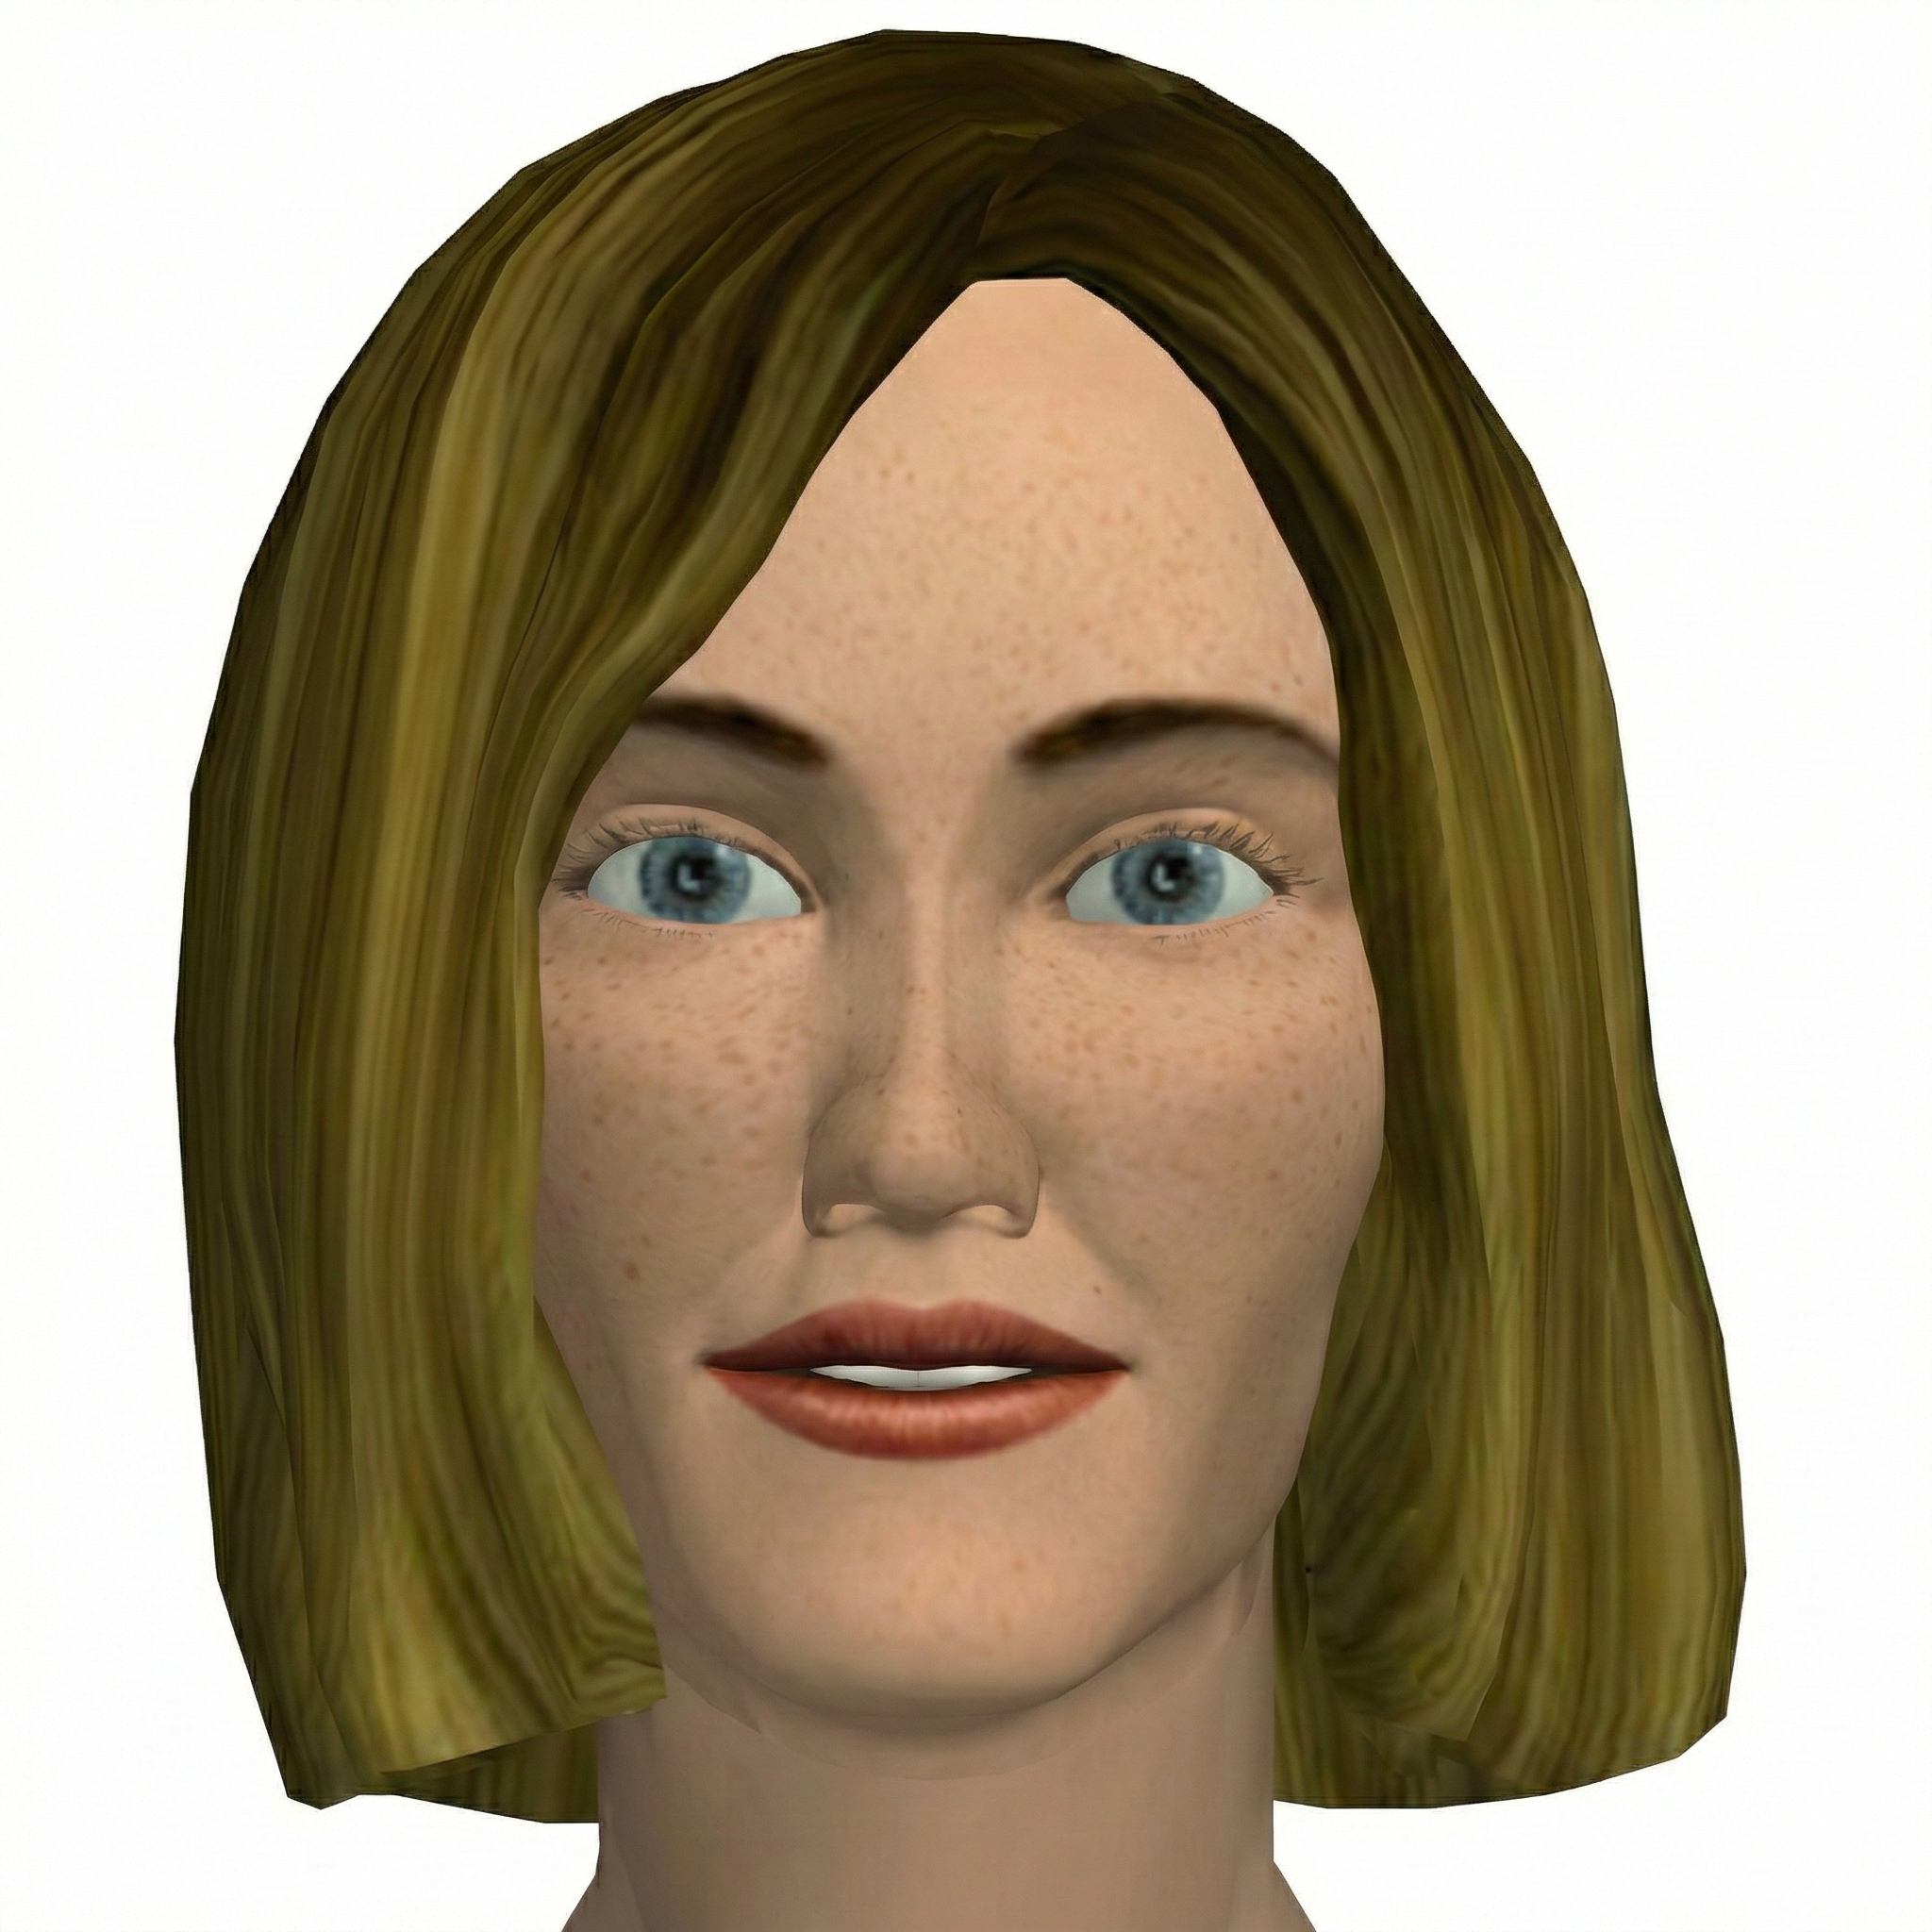
\includegraphics[width=\textwidth, height=4.5cm, keepaspectratio]{images/ch2/ochs2010.png}
    \caption{Agent expressif \citep{ochs2008}}
\end{subfigure}
\hfill
\begin{subfigure}[t]{0.3\textwidth}
    \vspace{0pt}
    \centering
    \includegraphics[width=\textwidth, height=4.5cm, keepaspectratio]{images/ch2/torre2019.png}
    \caption{Agent multimodal \citep{torre2019}}
\end{subfigure}
\caption{Évolution des agents pédagogiques sur trois décennies. De Steve (1997), premier agent pédagogique animé capable de gestes et d'expressions, aux agents expressifs modélisant des états émotionnels (2008), jusqu'aux systèmes contemporains intégrant expression multimodale et confiance (2019).}
\label{fig:evolution_agents}
\end{figure}

La distinction entre présence visuelle et comportement visuel éclaire les résultats précédents. La présence d'un corps à l'écran ne contribue pas de manière consistante à l'apprentissage, mais les comportements visuels spécifiques --- gestes, expressions, regard --- modulent la cognition par des mécanismes distincts. Les gestes déictiques --- pointer vers un élément pertinent --- dirigent l'attention vers l'information clé et améliorent l'apprentissage procédural \citep{davis2018, baylor2009}. Leur efficacité repose sur un mécanisme attentionnel, non social : ils orientent le regard et réduisent la recherche visuelle. Les expressions faciales agissent sur un registre différent. Elles favorisent l'adhésion aux messages et le changement d'attitude plutôt que l'acquisition de connaissances factuelles \citep{baylor2009}. Les gestes non liés au contenu améliorent néanmoins la rétention et le transfert, tout en augmentant le caractère humain perçu de l'agent, sans surcharge cognitive \citep{schneider2022}. Le regard direct constitue une exception. Le contact visuel augmente le temps de fixation sur l'agent, au détriment du contenu \citep{wilson2018, wang2017}. L'apprenant consacre des ressources cognitives au traitement du regard plutôt qu'au matériel pédagogique. Cet effet pourrait résulter d'un inconfort social ou d'une interférence attentionnelle non spécifique au regard.

Plusieurs méta-analyses permettent de hiérarchiser ces résultats. L'expressivité émotionnelle améliore davantage le transfert que la rétention \citep{wang2023-meta}. Cette asymétrie indique que les indices sociaux agissent sur le traitement profond --- réorganisation, application --- plutôt que sur l'encodage superficiel. La combinaison d'un design visuel et d'un rôle pédagogique défini produit des effets plus marqués que chaque dimension isolée \citep{marthasantoso2018}. L'apparence seule ne suffit pas. L'efficacité requiert une articulation entre persona et méthode pédagogique. Des résultats convergents émergent de revues systématiques récentes : la technologie sous-jacente et le type d'interaction comptent davantage que le degré de réalisme visuel \citep{dai2022-bx}.

Le profil motivationnel des agents présente cependant des limites. Les agents améliorent l'auto-efficacité et l'intérêt, mais n'ont pas d'effet détectable sur la motivation intrinsèque ni sur l'engagement \citep{gladstone2025}. Cette absence d'effet sur la motivation intrinsèque peut refléter plusieurs facteurs : une durée d'exposition insuffisante dans les protocoles expérimentaux, une mesure inadaptée au contexte technologique, ou un mécanisme distinct de ceux décrits par la SDT (cf.~\ref{subsec:sdt_cet}). La variabilité des résultats entre études indique que les bénéfices ne sont pas uniformes. Plusieurs modérateurs expliquent cette hétérogénéité. Les effets sont plus marqués chez les apprenants de 10--14 ans et chez les novices \citep{johnsonlester2016, zhang2024}. Cette tranche d'âge correspond au public cible de la thèse. Les disciplines STIM produisent des effets plus robustes que les sciences humaines \citep{alfaro2020}. L'enseignement de l'histoire, objet de cette recherche, se situe dans un domaine où les preuves sont moins solides. La stratégie pédagogique produit davantage d'effets que l'apparence. Les approches qui sollicitent activement l'apprenant --- questionnement divergent, scaffolding métacognitif, compétition ludique --- génèrent des gains d'apprentissage que le raffinement visuel de l'agent ne produit pas \citep{zhang2024}.

Ces résultats se heurtent à un plafond structurel propre aux agents classiques. Les agents scriptés fonctionnent à partir de réponses prédéfinies, sélectionnées dans un arbre de décision. Cette rigidité érode la présence sociale au fil de l'interaction \citep{schroeder2025}. L'apprenant finit par percevoir l'absence de contingence : l'agent ne répond pas de manière adaptée à ce qui a été dit. La co-construction au sens du cadre ICAP (cf.~\ref{subsec:icap}) suppose que chaque contribution s'appuie sur la précédente. Les systèmes scriptés ne fournissent pas cette adaptation sémantique en temps réel. À cette limite technologique s'ajoute un constat perceptuel. Les résultats précédents indiquent que les agents 2D tendent à produire de meilleurs résultats que les agents 3D et que le réalisme visuel ne semble pas déterminer à lui seul l'efficacité pédagogique. La relation entre l'apparence de l'agent et la réponse de l'apprenant ne suit pas un gradient linéaire.


\subsection{Les ruptures de présence : la vallée de l'étrange}
\label{subsec:uncanny_valley}

La relation entre réalisme de l'agent et réponse affective de l'utilisateur n'est pas linéaire. La vallée de l'étrange (\textit{uncanny valley}) désigne une zone où l'affinité, après avoir crû avec le degré de ressemblance humaine, chute brutalement avant de remonter lorsque l'agent devient indiscernable d'un humain \citep{mori2012}. Cette vallée n'est pas un artefact de laboratoire : elle se manifeste dans les jugements de confiance et d'attractivité portés sur des visages numériques dont le réalisme varie systématiquement \citep{mcdonnell2012}. Le mécanisme proposé repose sur un conflit perceptif : un agent presque humain active les attentes propres aux interactions humaines, mais les violations subtiles --- un mouvement oculaire trop lent, une micro-expression absente, un sourire asymétrique --- produisent un malaise que les agents stylisés ne déclenchent pas, précisément parce qu'ils n'activent pas ces attentes.

La théorie des violations d'attentes (\textit{Expectancy Violation Theory}) fournit le cadre qui explique ce mécanisme au-delà de la seule apparence visuelle \citep{burgoon2015}. Toute interaction repose sur des attentes implicites concernant le comportement de l'interlocuteur. Une violation positive --- un agent qui répond mieux que prévu --- renforce l'engagement. Une violation négative --- un comportement incohérent avec les indices émis par l'agent --- produit un inconfort qui détourne les ressources cognitives du contenu vers l'évaluation de la source. Un agent dont le réalisme comportemental ne correspond pas aux attentes créées par son apparence tend à susciter davantage d'inconfort qu'un agent aux capacités modestes qui n'active pas ces attentes \citep{groom2009, haresamudram2024}. L'alignement multimodal --- la cohérence entre apparence visuelle, qualité vocale et comportement gestuel --- prédit la réponse affective de l'utilisateur mieux que le réalisme de chaque modalité prise isolément \citep{alimardani2024}. Ces attentes dépendent en outre du contexte : un agent pédagogique n'est pas évalué selon les mêmes critères qu'un agent de divertissement, et le seuil de tolérance aux incohérences varie avec le rôle attribué à l'agent \citep{torre2019}.

La leçon convergente de ces travaux est que le réalisme n'est pas un objectif de design en soi. Un agent trop réaliste pour son niveau de comportement peut produire une distraction cognitive susceptible de réduire l'apprentissage \citep{parmar2022}. Les agents au style cartoon et les agents photoréalistes produisent des effets d'apprentissage comparables, mais les premiers génèrent moins de distraction et réduisent le risque de tomber dans la vallée de l'étrange \citep{li2024}. Le principe de design qui en découle privilégie la cohérence sur le réalisme : viser un niveau de ressemblance humaine que le comportement de l'agent --- verbal, vocal et gestuel --- peut soutenir sans rupture. Les IA génératives modifient cette équation. La fluence du langage naturel et la capacité d'adaptation contextuelle augmentent la cohérence comportementale, ce qui permet de soutenir des niveaux de réalisme plus élevés sans déclencher de violations d'attentes. Cette avancée ouvre de nouvelles possibilités, mais introduit simultanément de nouveaux risques que les sections suivantes examineront.



%%%%%%%%%%%%%%%%%%%%%%%%%%%%%%%%%%%%%%%%%%%%%%%%%%%%%%%%%%%%%%%%%
% 2.4. L'Émergence des IA Génératives en Éducation
%%%%%%%%%%%%%%%%%%%%%%%%%%%%%%%%%%%%%%%%%%%%%%%%%%%%%%%%%%%%%%%%%
\section{L'Émergence des IA Génératives en Éducation}
\label{sec:ia_generatives}

\section{L'émergence des IA génératives en éducation}
\label{sec:ia_generatives}

\subsection{Des agents scriptés aux agents génératifs : le saut qualitatif}
\label{subsec:agents_scriptes_generatifs}

Les agents pédagogiques classiques fonctionnent selon une logique de scripts prédéfinis. L'apprenant pose une question ; le système la compare à une base de patterns ; il sélectionne une réponse dans un arbre de décision. Cette architecture impose deux contraintes. La couverture dépend du nombre de cas anticipés par les concepteurs. La contingence conversationnelle reste superficielle, car l'agent ne construit pas sa réponse à partir du contenu sémantique de l'échange. Les revues systématiques confirment ce diagnostic : les agents scriptés produisent des effets positifs mais modestes, et leur efficacité décroît avec la durée d'interaction \citep{schroeder2025, veletsianos2013}. L'apprenant détecte progressivement l'absence de véritable adaptation, ce qui érode la présence sociale (cf.~\ref{subsec:incarnation_agence_sociale}).

Les grands modèles de langage (LLM, \textit{Large Language Models}) reposent sur une architecture radicalement différente. Un LLM est un réseau de neurones entraîné sur des corpus massifs de textes à prédire le mot suivant d'une séquence. L'entraînement ajuste des milliards de paramètres pour capturer les régularités statistiques du langage. Le modèle n'apprend pas des règles explicites : il apprend des distributions de probabilités sur des séquences de tokens. À l'inférence, le modèle génère du texte token par token, chaque prédiction conditionnée par le contexte précédent. Cette génération autoregressive produit un discours fluide et cohérent sans recourir à des scripts prédéfinis \citep{vaswani2017, brown2020}.

Cette architecture confère aux LLM une propriété centrale : la génération contextuelle. Le modèle produit des réponses adaptées au contenu spécifique de l'échange, non sélectionnées dans un répertoire fixe. De cette propriété découlent deux capacités dérivées. La flexibilité stylistique permet d'ajuster le registre, le niveau de détail et le ton en fonction du profil inféré de l'utilisateur. La capacité de raisonnement apparent permet de décomposer des problèmes et d'expliquer des étapes de raisonnement \citep{wei2022}. Ces capacités convergent vers un même effet : une adaptation en temps réel qui positionne les LLM comme des outils prometteurs pour l'accompagnement pédagogique \citep{pataranutaporn2021, yan2024}.

Ces capacités trouvent des applications dans l'enseignement de l'histoire, un domaine où la narration et le dialogue avec des figures du passé présentent un potentiel pédagogique spécifique. Des plateformes expérimentales intègrent désormais des personnages non-joueurs génératifs dans des simulations historiques \citep{park2025}, tandis que d'autres exploitent l'ingénierie de prompt comme activité d'apprentissage à part entière \citep{lim2025}. Ces prototypes démontrent la faisabilité technique de l'approche. Leur évaluation reste cependant limitée : échantillons restreints, mesures principalement perceptuelles, absence de suivi longitudinal. La question de l'efficacité pédagogique réelle demeure ouverte.

L'évolution des médias synthétiques amplifie cette transformation. Les réseaux antagonistes génératifs (GANs) et les modèles de diffusion permettent de créer des visages photoréalistes, de cloner des voix et de générer des animations faciales synchronisées avec la parole \citep{whittaker2020}. Un instructeur virtuel peut désormais présenter une apparence humaine convaincante et une voix indiscernable d'un enregistrement réel. Ces agents hyperréalistes évitent la vallée de l'étrange et sont perçus comme attractifs \citep{xu2025a}. Cette attractivité n'est pas neutre : elle peut favoriser l'engagement, mais aussi réduire la distance critique que l'apprenant maintient face à une source d'information. La fluence comportementale des LLM --- leur capacité à maintenir une conversation naturelle --- soutient des niveaux de réalisme visuel que les systèmes scriptés ne pouvaient pas accompagner.

La convergence de ces deux avancées --- génération de langage naturel et synthèse médiatique --- produit une nouvelle équation. D'un côté, un moteur conversationnel capable de générer un discours parfaitement articulé. De l'autre, une interface visuelle hyperréaliste pour l'incarner. Cette combinaison permet de créer des agents qui maintiennent la présence sociale au-delà des premières minutes d'interaction, précisément parce qu'ils produisent des réponses contextuellement pertinentes plutôt que des sélections dans un catalogue. La co-construction au sens du cadre ICAP (cf.~\ref{subsec:icap}) devient techniquement possible : chaque contribution de l'agent peut s'appuyer sur la précédente et la transformer.

Cette avancée ouvre de nouvelles possibilités pédagogiques. Les agents génératifs peuvent fournir un feedback individualisé, adapter leurs explications au niveau de l'apprenant et maintenir un dialogue soutenu sur des sujets complexes. Certaines études rapportent des performances d'apprentissage comparables à celles obtenues avec des instructeurs humains \citep{leiker2023, lim2024}. Cette comparabilité mérite cependant d'être interrogée : elle repose sur des mesures immédiates, des échantillons restreints et des contextes expérimentaux qui limitent la généralisation. L'intégration de techniques de récupération augmentée (RAG, \textit{Retrieval-Augmented Generation}) permet d'ancrer les réponses dans des sources vérifiées, réduisant partiellement le risque d'erreurs factuelles \citep{lewis2020}.

Cette capacité nouvelle introduit simultanément des risques inédits. La fluence linguistique des LLM ne garantit pas l'exactitude de leur contenu. La section suivante examine comment cette fluence peut servir la personnalisation de l'apprentissage, avant d'aborder le défi épistémique que posent les hallucinations.


\subsection{La personnalisation de l'apprentissage}
\label{subsec:personnalisation_apprentissage}

Les capacités de génération contextuelle décrites en~\ref{subsec:agents_scriptes_generatifs} ouvrent une forme de personnalisation inaccessible aux systèmes à règles fixes. Un LLM adapte en temps réel la formulation, le registre et le niveau de détail au fil de l'échange, sans que le concepteur ait à anticiper chaque cas. Cette adaptation sémantique produit un effet asymétrique : la personnalisation du contenu par un LLM --- phrases et récits ajustés au profil de l'apprenant --- améliore la motivation intrinsèque, mais n'affecte pas la performance d'apprentissage mesurée par des tests de compréhension \citep{leong2024}. L'adaptation agit donc sur l'intérêt perçu, pas sur le traitement cognitif du contenu. Ce pattern --- perception améliorée, apprentissage inchangé --- se reproduit dans les travaux présentés ci-après.

Au-delà du contenu, la personnalisation peut porter sur l'agent lui-même. L'utilisation de personnalités admirées comme instructeurs vidéo améliore la motivation et les émotions positives, sans modifier les scores d'apprentissage \citep{pataranutaporn2022}. Le passage au format interactif accentue cet effet : lorsque les apprenants dialoguent avec l'instructeur virtuel via un chat textuel, l'engagement augmente par rapport au visionnage passif, les scores d'apprentissage restant équivalents \citep{prasongpongchai2024}. L'interactivité ajoute ainsi une dimension que la vidéo seule ne capture pas. L'effet atteint son maximum lorsque la connexion repose sur une relation déjà établie. La comparaison entre un chatbot textuel, une mascotte 3D et un deepfake de l'enseignant réel des élèves montre que la familiarité préexistante avec la personne représentée augmente la confiance et la compétence perçue de l'agent \citep{tan2025}. La gradation est nette : image d'une figure admirée, puis interaction avec cette figure, puis relation préexistante avec la personne imitée --- chaque étape renforce la perception sans que l'apprentissage mesuré ne suive. Les comparaisons directes entre agents génératifs et instructeurs humains confirment ce constat : l'équivalence rapportée porte sur des mesures immédiates dans des contextes contrôlés, non sur une reproduction du processus d'enseignement humain \citep{leiker2023, lim2024}.

Le mécanisme sous-jacent relève d'un transfert de crédibilité : l'apprenant reporte sur l'agent la confiance qu'il accorde déjà à la personne représentée, comme le montre la gradation décrite ci-dessus. L'apparence humaine agit en outre comme un prédicteur de l'utilité perçue, un effet médié par l'interactivité attendue plutôt que par la ressemblance elle-même \citep{lin2024}. Cette dissociation entre perception et apprentissage, déjà documentée pour les agents classiques (cf.~\ref{subsec:incarnation_agence_sociale}), pose un problème de conception. L'attrait visuel de l'agent peut détourner des ressources attentionnelles du contenu vers l'interface, un phénomène observé y compris avec des instructeurs humains filmés (cf.~\ref{subsec:incarnation_agence_sociale}). Cette tension entre engagement perçu et traitement cognitif s'accentue lorsque l'agent incarne une figure historique.

Des institutions culturelles déploient déjà des agents conversationnels incarnant des figures disparues. Au Dalí Museum de St. Petersburg, l'installation \textit{Ask Dalí}\footnote{\url{https://thedali.org/exhibit/ask-dali/}} permet aux visiteurs de converser avec une reconstruction de Salvador Dalí via un téléphone-homard, objet iconique de son \oe{}uvre surréaliste (voir Figure~\ref{fig:ask_dali}). Le système, alimenté par GPT-4 et une synthèse vocale entraînée sur des archives audio, produit des réponses reflétant la personnalité de l'artiste. Au Musée d'Orsay, l'expérience \textit{Hello Vincent}\footnote{\url{https://www.musee-orsay.fr/fr/articles/numerique-bonjour-vincent-275618}} propose une interaction avec Van Gogh appuyée sur un corpus de près de 900 lettres validé par un historien de l'art (voir Figure~\ref{fig:vangogh_museum}). Ces déploiements marquent le passage du prototype de recherche au grand public. Ils révèlent aussi une tension : le cadre muséal vise la médiation culturelle et l'engagement émotionnel, tandis que le cadre scolaire exige l'exactitude factuelle et l'apprentissage conceptuel.

\begin{figure}[htbp]
    \centering
    \includegraphics[width=0.7\textwidth]{images/ch2/dali.png}
    \caption{Installation \textit{Ask Dalí} au Dalí Museum de St. Petersburg. Les visiteurs conversent avec une reconstruction IA de Salvador Dalí via un téléphone-homard. La citation murale --- « I do not understand why, when I ask for a grilled lobster in a restaurant, I am never served a cooked telephone » --- illustre l'humour surréaliste que le système cherche à reproduire.}
    \label{fig:ask_dali}
\end{figure}

\begin{figure}[htbp]
    \centering
    
\includegraphics[width=0.7\textwidth]{images/ch2/vangogh.png}
    \caption{Représentation numérique de Vincent van Gogh dans l'expérience \textit{Hello Vincent} au Musée d'Orsay. Le visiteur converse avec l'artiste pendant qu'il peint son célèbre \textit{Champ de blé aux corbeaux}, l'IA s'appuyant sur un corpus de près de 900 lettres.}
    \label{fig:vangogh_museum}
\end{figure}

Plusieurs travaux explorent cette personnification dans un cadre expérimental. Des participants adultes conversant avec des reconstructions de Leonardo Da Vinci ou Murasaki Shikibu rapportent une motivation et une efficacité d'apprentissage perçue supérieures à la lecture seule \citep{pataranutaporn2023} (voir Figure~\ref{fig:living_memories}). Des collégiens dialoguant avec Napoléon ou Alexandre le Grand montrent une amélioration de l'empathie historique et des capacités d'auto-réflexion \citep{kim2025}. Les variables mesurées --- motivation, empathie, engagement --- relèvent toutefois du registre affectif. L'apprentissage factuel, la compréhension conceptuelle et la rétention à long terme restent largement inexplorés, conformément au pattern identifié plus haut. L'effet optimal survient lorsque l'interaction complète les sources textuelles plutôt que de s'y substituer \citep{pataranutaporn2023}. La valeur pédagogique de ces agents semble résider dans la complémentarité, non dans la substitution.

\begin{figure}[htbp]
    \centering
    \includegraphics[width=0.8\textwidth]{images/ch2/living-memories-talking.png}
    \caption{Interface du projet \textit{Living Memories} \citep{pataranutaporn2023}. L'utilisateur converse avec une reconstruction de Leonardo Da Vinci, qui se présente et répond aux questions. Le système combine GPT-3 et un extracteur sémantique pour générer des réponses cohérentes avec le personnage historique.}
    \label{fig:living_memories}
\end{figure}

La personnalisation par l'apparence soulève également des questions que la littérature commence à explorer \citep{danry2022}. Le consentement de la personne représentée ne peut être obtenu lorsqu'il s'agit de figures historiques décédées. Les effets d'une exposition prolongée à des représentations synthétiques sur la perception de l'authenticité restent inconnus. La confusion entre l'agent et la personne qu'il imite constitue un risque, en particulier pour de jeunes apprenants. Au-delà de ces enjeux liés à l'apparence de l'agent, la fiabilité du contenu qu'il produit constitue un problème distinct, examiné dans la section suivante.


\subsection{Fiabilité et hallucinations : le défi épistémique}
\label{subsec:fiabilite_hallucinations}

Les LLM génèrent du texte en prédisant le token le plus probable étant donné le contexte. Cette génération est intrinsèquement stochastique : le même prompt peut produire des réponses différentes. Le modèle ne dispose pas d'une représentation du monde qu'il consulterait pour vérifier ses énoncés. Il produit des séquences statistiquement plausibles, sans mécanisme interne de validation factuelle. Cette architecture explique le phénomène des hallucinations : la génération d'informations factuellement incorrectes présentées avec une apparente certitude. Ces hallucinations peuvent concerner des faits (dates erronées, événements inventés), la fidélité au contexte d'entrée ou la validité logique du raisonnement \citep{zhang2025}.

Quelle que soit leur forme, ces hallucinations partagent une caractéristique commune : le modèle les produit avec la même assurance apparente que ses énoncés corrects. Aucun signal textuel --- ni hésitation, ni marqueur d'incertitude, ni avertissement --- ne distingue le vrai du faux \citep{zhang2025}.

Cette absence de marqueurs d'incertitude pose un problème spécifique en contexte pédagogique. Le discours des LLM est structuré, cohérent et exempt d'hésitations, ce qui le rend indiscernable, en surface, d'un discours fiable. Des inexactitudes subtiles présentées avec une apparente autorité constituent ce que la littérature qualifie de « discours négligent » (\textit{negligent discourse}) \citep{wachter2024}. L'apprenant ne dispose d'aucun indice formel pour distinguer les énoncés fiables des énoncés erronés --- et les indices disponibles (structure, cohérence, assurance) sont uniformément rassurants. Une étude auprès de collégiennes confrontées à ChatGPT illustre cette vulnérabilité : 59\,\% des réponses incorrectes sont jugées correctes, une confiance excessive attribuée en partie à la « légitimité esthétique » du discours généré \citep{solyst2024}.

Ce problème prend une forme particulière en histoire. Le discours historique mobilise des récits, des personnages et des enchaînements causaux qui se prêtent naturellement à la narration. Un LLM peut générer un récit historique cohérent sur le plan narratif tout en contenant des erreurs factuelles. La plausibilité narrative tend à masquer l'inexactitude factuelle. Une étude de faisabilité sur la reconstruction conversationnelle de Joseph Lister\footnote{\url{https://fr.wikipedia.org/wiki/Joseph_Lister}}, chirurgien anglais du \textsc{xix}\textsuperscript{e} siècle, en fournit un exemple \citep{dacsta2025}. L'agent, doté d'un système de récupération augmentée, produit des réponses fidèles à la voix historique du personnage, mais les évaluations détectent des lacunes dans le cadrage temporel, des embellissements occasionnels et des événements incorrectement situés. L'apprenant peut accepter ces informations erronées sans les questionner, précisément parce qu'elles s'insèrent dans une trame cohérente.

Ce cas illustre une difficulté structurelle. Les distorsions ne relèvent pas d'erreurs grossières : elles s'insèrent dans un discours par ailleurs cohérent et engageant. Seul un expert du domaine peut les identifier. Ce constat ne se limite pas à l'histoire : dans un contexte moteur, des instructions hallucinées par un LLM ont conduit à des performances significativement inférieures à celles d'un enseignement traditionnel \citep{qiu2024}. La récupération augmentée (RAG, \textit{Retrieval-Augmented Generation}) --- qui ancre les réponses dans des sources vérifiées \citep{lewis2021} --- réduit le risque d'hallucinations flagrantes, mais ne garantit pas l'exactitude des nuances, des interprétations et du cadrage temporel. En histoire, ces nuances constituent souvent l'essentiel de la compréhension disciplinaire.

Le problème dépasse la seule production de contenu erroné. L'absence de signaux d'erreur rend la détection des hallucinations tributaire de connaissances que l'apprenant en situation d'apprentissage ne possède pas encore. Les mécanismes cognitifs qui expliquent pourquoi cette vulnérabilité persiste même face à des erreurs identifiables font l'objet de la section suivante.


